\documentclass{article}
\usepackage[margin=0.2in,paperwidth=9in,paperheight=4.8in]{geometry}
\pagestyle{empty}
\usepackage{amsmath,amssymb}
\usepackage{tikz}
\usetikzlibrary{shapes.geometric, arrows.meta, positioning, calc}

\begin{document}
\noindent
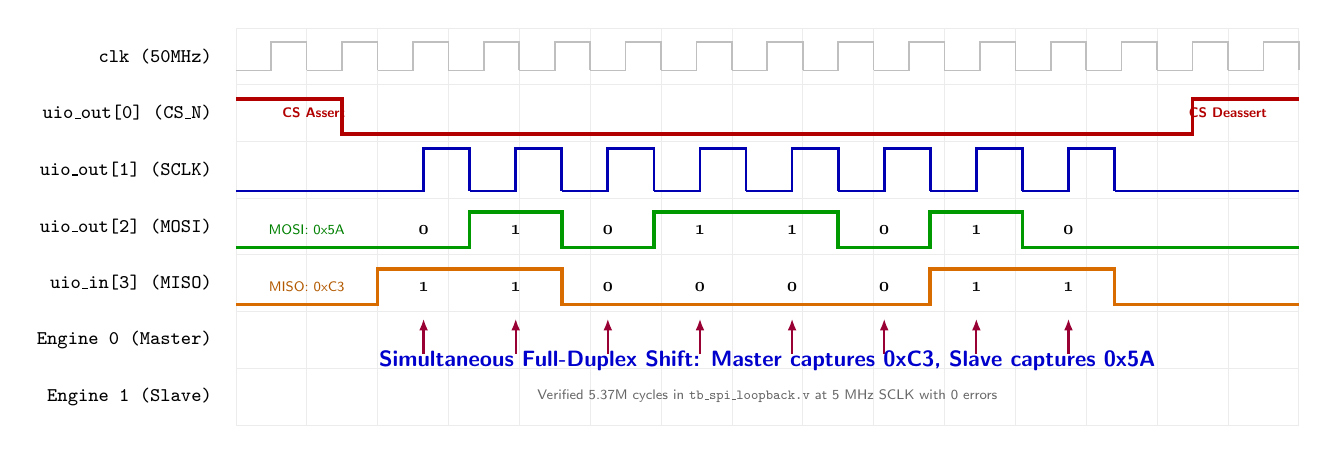
\begin{tikzpicture}[
    scale=0.9,
    clock/.style={line width=1pt, blue!70!black},
    sig/.style={line width=1.3pt, red!70!black},
    data/.style={line width=1.3pt, green!60!black},
    bus/.style={line width=1.3pt, purple!80!black},
    txt/.style={font=\scriptsize\sffamily},
    lbl/.style={font=\scriptsize\ttfamily, anchor=east}
]

% Background grid
\draw[help lines, color=gray!15, ystep=0.8, xstep=1] (0, 0) grid (15, 5.6);

% Labels
\node[lbl] at (-0.2, 5.2) {clk (50MHz)};
\node[lbl] at (-0.2, 4.4) {uio\_out[0] (CS\_N)};
\node[lbl] at (-0.2, 3.6) {uio\_out[1] (SCLK)};
\node[lbl] at (-0.2, 2.8) {uio\_out[2] (MOSI)};
\node[lbl] at (-0.2, 2.0) {uio\_in[3] (MISO)};
\node[lbl] at (-0.2, 1.2) {Engine 0 (Master)};
\node[lbl] at (-0.2, 0.4) {Engine 1 (Slave)};

% Master Clock
\foreach \i in {0,...,14} {
    \draw[line width=0.6pt, gray!50] (\i, 5.0) -- (\i+0.5, 5.0) -- (\i+0.5, 5.4) -- (\i+1.0, 5.4) -- (\i+1.0, 5.0);
}

% CS_N (Active-low chip select)
\draw[sig] (0, 4.6) -- (1.5, 4.6) -- (1.5, 4.1) -- (13.5, 4.1) -- (13.5, 4.6) -- (15, 4.6);
\node[txt, font=\tiny\bfseries\sffamily, red!70!black] at (1.1, 4.4) {CS Assert};
\node[txt, font=\tiny\bfseries\sffamily, red!70!black] at (14.0, 4.4) {CS Deassert};

% SCLK (Mode 0: CPOL=0, idle low, 8 clocks)
\draw[clock] (0, 3.3) -- (2.0, 3.3);
\foreach \i in {0,...,7} {
    \draw[clock] (2.0 + \i*1.3, 3.3) -- (2.0 + \i*1.3 + 0.65, 3.3) -- (2.0 + \i*1.3 + 0.65, 3.9) -- (2.0 + \i*1.3 + 1.3, 3.9) -- (2.0 + \i*1.3 + 1.3, 3.3);
}
\draw[clock] (12.4, 3.3) -- (15, 3.3);

% MOSI: Master sends 0x5A = 01011010 (MSB first)
% Bits: 0, 1, 0, 1, 1, 0, 1, 0
\draw[data] (0, 2.5) -- (2.0, 2.5) % bit 7 = 0
           -- (3.3, 2.5) -- (3.3, 3.0) -- (4.6, 3.0) -- (4.6, 2.5) % bit 6 = 1
           -- (5.9, 2.5) -- (5.9, 3.0) -- (7.2, 3.0) % bit 5 = 0, bit 4 = 1
           -- (8.5, 3.0) -- (8.5, 2.5) -- (9.8, 2.5) % bit 3 = 1, bit 2 = 0
           -- (9.8, 3.0) -- (11.1, 3.0) -- (11.1, 2.5) % bit 1 = 1, bit 0 = 0
           -- (12.4, 2.5) -- (15, 2.5);

% MOSI Labels
\foreach \x/\b in {2.65/0, 3.95/1, 5.25/0, 6.55/1, 7.85/1, 9.15/0, 10.45/1, 11.75/0} {
    \node[txt, font=\tiny\bfseries] at (\x, 2.75) {\b};
}
\node[txt, font=\tiny\sffamily, green!50!black] at (1.0, 2.75) {MOSI: 0x5A};

% MISO: Slave sends 0xC3 = 11000011 (MSB first)
% Bits: 1, 1, 0, 0, 0, 0, 1, 1
\draw[data, color=orange!85!black] (0, 1.7) -- (2.0, 1.7) -- (2.0, 2.2)
           -- (4.6, 2.2) -- (4.6, 1.7) -- (9.8, 1.7) % bit 7=1, bit 6=1, bits 5..2=0
           -- (9.8, 2.2) -- (12.4, 2.2) -- (12.4, 1.7) -- (15, 1.7); % bits 1..0=1

% MISO Labels
\foreach \x/\b in {2.65/1, 3.95/1, 5.25/0, 6.55/0, 7.85/0, 9.15/0, 10.45/1, 11.75/1} {
    \node[txt, font=\tiny\bfseries] at (\x, 1.95) {\b};
}
\node[txt, font=\tiny\sffamily, orange!70!black] at (1.0, 1.95) {MISO: 0xC3};

% Sampling Strobes on SCLK edges (Mode 0: sample on rising edge)
\foreach \i in {0,...,7} {
    \draw[-{Latex[length=1.5mm]}, line width=0.8pt, purple!80!black] (2.0 + \i*1.3 + 0.65, 1.0) -- (2.0 + \i*1.3 + 0.65, 1.5);
}

% State summary
\node[txt, font=\footnotesize\bfseries\sffamily, text=blue!80!black] at (7.5, 0.9) {Simultaneous Full-Duplex Shift: Master captures 0xC3, Slave captures 0x5A};
\node[txt, font=\tiny\sffamily, text=gray!80!black] at (7.5, 0.4) {Verified 5.37M cycles in \texttt{tb\_spi\_loopback.v} at 5 MHz SCLK with 0 errors};

\end{tikzpicture}
\end{document}
